\documentclass[11pt,a4paper]{article}
\usepackage{tikz}
\usetikzlibrary{arrows.meta,positioning}
\usepackage{tabularx}
\usepackage{amsmath,amssymb,amsthm}
\usepackage{geometry}
\geometry{margin=1in}
\usepackage{hyperref}
\usepackage{graphicx}
\usepackage{setspace}
\onehalfspacing

\title{\textbf{Paper B-10: Autonomous Systems:\\ A Constraint-Driven Flux Dynamics (CDFD) Perspective}}
\author{Steve Bico Mujjabi, MD\\
\small Independent Researcher\\
\small Founder, Vura Labs\\
\small Kampala, Uganda\\
\small ORCID: 0009-0001-0556-5516}
\date{August 2026}

\begin{document}
\maketitle

% BEGIN SHARED-METHODS POINTER
\noindent\textit{Shared Part IV notation and evidence boundaries are defined in \path{PART_IV_METHODS_AND_CLAIM_BOUNDARY.md}. This paper states only its local observables, comparison, and failure conditions.}
% END SHARED-METHODS POINTER


\begin{abstract}
This paper develops a falsifiable CDFD/AFL model of Autonomous Systems. It maps sensor input, task demand, environmental change, and control goals to driving flux $\Phi$, actuation, compute, energy, uncertainty, and safety limits to active constraint $C$, planning, replanning, fallback, learning, and human oversight to responsiveness $S$, and learned policy, world model, event history, and accumulated wear to structural memory $M_s$. The target outcome is task success, robustness, safety margin, and recovery, tested against simulator traces, field logs, interventions, near misses, and distribution shifts. The paper treats universality as a shared model architecture rather than an assertion that unlike systems have the same material mechanism. It states the negative result that would make the mapping unnecessary and places the domain claim inside the cumulative CDFD programme and its reproducible runtime boundary.
\end{abstract}

\section{Introduction}

A robot navigating a busy city street is a thermodynamic engine attempting to process a chaotic stream of informational and physical variables. When a self-driving car encounters a novel situation (e.g., an unpredictable pedestrian), it must instantly adjust its velocity and trajectory.

If the robot's programming is too rigid, it will simply freeze in place, unable to compute a safe path. In CDFD terms, the robot has encountered an infinite topological constraint.

\section{The Robotic Adaptive Surface}
We govern autonomous behavior using the Adaptive Operating Ratio:
\begin{equation}
    \Psi_s = \left( \frac{\Phi}{C} \right) \cdot S \cdot M_s
\end{equation}

For an autonomous agent (like a drone or self-driving car):
\begin{itemize}
    \item \textbf{Flux ($\Phi$)}: The rate of sensory data ingestion (LIDAR, cameras) and the corresponding kinetic motor output (speed/movement).
    \item \textbf{Constraint ($C$)}: The physical obstacles in the environment, combined with the hardcoded safety limits programmed into the robot's control matrix.
    \item \textbf{Responsiveness ($S$)}: The computational speed of the inference engine and the physical agility of the robotic actuators.
    \item \textbf{Memory ($M_s$)}: The trained neural network weights and prior mapping data. If the robot relies too heavily on a pre-computed map, its memory is highly locked, making it vulnerable to sudden environmental changes.
\end{itemize}

\subsection{The Algorithmic Freeze State}
In a perfectly mapped environment, the robot flows smoothly. The sensory flux $\Phi$ is easily processed against known constraints $C$, maintaining $\Psi_s \approx 1$.

Consider a scenario where the environment suddenly changes (e.g., a construction zone blocks the mapped road). The external constraint $C$ spikes dramatically. If the robot's memory ($M_s$) dictates that it must strictly follow the pre-computed path, it cannot find a valid mathematical solution. The effective responsiveness $S$ drops to zero. The adaptive ratio crashes ($\Psi_s \ll 1$).

The robot enters a "freeze" state, simply halting all kinetic flux $\Phi$. It has suffered a topological stroke. To achieve true autonomy, the robotic architecture must possess an internal mechanism to instantly discard its restrictive memory ($M_s$) when $C$ spikes, allowing it to dynamically explore novel, low-constraint topological pathways without breaking its core safety parameters.



\section{Measurement Layer}

% BEGIN PART IV MAJOR CROSS-DOMAIN UPGRADE
\section{Cross-Domain Model Upgrade: Mechanism, Scale, and Tests}

\subsection{Observable Translation}

The paper-specific translation begins with an observable chain rather than a
verbal analogy. For Autonomous Systems, the proposed drive is sensor input, task demand, environmental change, and control goals.
The active limitation is actuation, compute, energy, uncertainty, and safety limits. Responsiveness is carried by
planning, replanning, fallback, learning, and human oversight, while retained state is represented by
learned policy, world model, event history, and accumulated wear. The outcome to explain is task success, robustness, safety margin, and recovery.

\begin{table}[htbp]
\centering
\small
\caption{Operational CDFD/AFL map for Paper B-10.}
\begin{tabularx}{\textwidth}{|l|X|X|}
\hline
\textbf{Term} & \textbf{Paper-specific observable meaning} & \textbf{Measurement question} \\
\hline
$\Phi$ & sensor input, task demand, environmental change, and control goals & What rate, load, gradient, or demand enters the focal system? \\
\hline
$C$ & actuation, compute, energy, uncertainty, and safety limits & Which measured bottleneck limits transfer, function, or recovery? \\
\hline
$S$ & planning, replanning, fallback, learning, and human oversight & Which process changes effective capacity or reroutes the load? \\
\hline
$M_s$ & learned policy, world model, event history, and accumulated wear & Which retained state makes equal present loads produce different futures? \\
\hline
$Y$ & task success, robustness, safety margin, and recovery & Which outcome is predicted out of sample, with uncertainty? \\
\hline
\end{tabularx}
\end{table}

\begin{figure}[htbp]
\centering
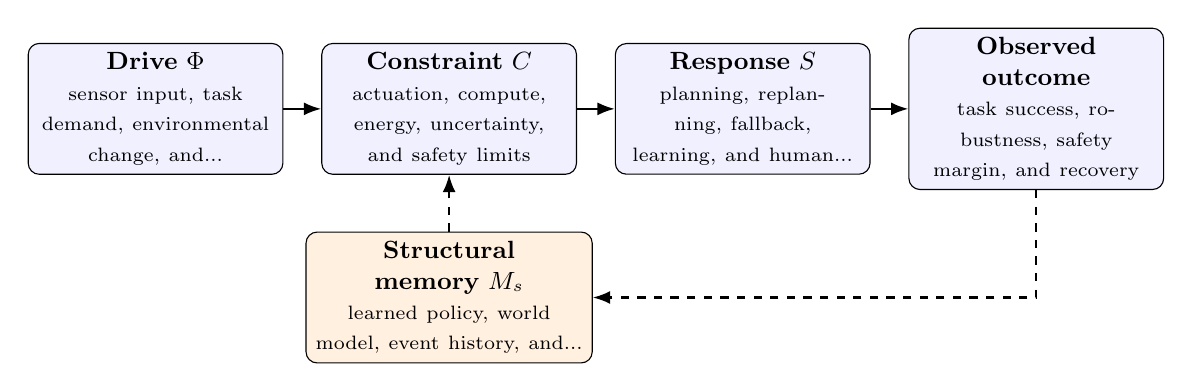
\begin{tikzpicture}[
    node distance=0.48cm,
    every node/.style={font=\small},
    box/.style={draw, rounded corners, align=center, minimum height=1.45cm, text width=3.0cm, fill=blue!6},
    memory/.style={draw, rounded corners, align=center, minimum height=1.25cm, text width=3.4cm, fill=orange!12},
    flow/.style={-{Latex[length=2.2mm]}, thick},
    feedback/.style={-{Latex[length=2.2mm]}, thick, dashed}
]
\node[box] (drive) {\textbf{Drive $\Phi$}\\\scriptsize sensor input, task demand, environmental change, and...};
\node[box, right=of drive] (constraint) {\textbf{Constraint $C$}\\\scriptsize actuation, compute, energy, uncertainty, and safety limits};
\node[box, right=of constraint] (response) {\textbf{Response $S$}\\\scriptsize planning, replanning, fallback, learning, and human...};
\node[box, right=of response] (outcome) {\textbf{Observed outcome}\\\scriptsize task success, robustness, safety margin, and recovery};
\node[memory, below=0.72cm of constraint] (memory) {\textbf{Structural memory $M_s$}\\\scriptsize learned policy, world model, event history, and...};
\draw[flow] (drive) -- (constraint);
\draw[flow] (constraint) -- (response);
\draw[flow] (response) -- (outcome);
\draw[feedback] (outcome.south) |- (memory.east);
\draw[feedback] (memory.north) -- (constraint.south);
\end{tikzpicture}
\caption{Paper B-10 observable CDFD/AFL architecture for Autonomous Systems. Solid arrows give the proposed forward chain; dashed arrows make history-dependent feedback explicit.}
\label{fig:b10-architecture}
\end{figure}

\subsection{Paper-Specific Causal Hypothesis}

For this paper, the hypothesized causal sequence is specific. A change in
sensor input, task demand, environmental change, and control goals arrives faster than planning, replanning, fallback, learning, and human oversight can compensate.
This raises or redistributes actuation, compute, energy, uncertainty, and safety limits. If the load persists,
the retained state encoded by learned policy, world model, event history, and accumulated wear changes the next response, so a later event of equal
magnitude can produce a different trajectory in task success, robustness, safety margin, and recovery. The
scientific task is to estimate that sequence against the best ordinary model of
the domain, not merely to redescribe the outcome after it occurs.

\subsection{Cross-Scale Translation Without Mechanistic Erasure}

For the engineered systems family, the cross-domain translation compares demand, designed capacity, feedback control, dependency topology, and accumulated technical state. The strongest engineering use is prospective: the mapping must identify a bottleneck, a control action, or a recovery signature before the failure occurs. \cite{BarabasiAlbert1999,WattsStrogatz1998,Shannon1948,BakTangWiesenfeld1987}
The required scale declaration for this paper is milliseconds to decades; controllers to autonomous fleets. At short
scales, the key question is whether the incoming drive is transmitted,
buffered, or diverted. At intermediate scales, response changes effective
capacity and network exposure. At long scales, retained structure can alter the
state space itself. A result is genuinely cross-scale only when the aggregation
rule is stated and the same conclusion is not an artifact of averaging.

\subsection{Evidence Ladder and Discriminating Tests}

\begin{table}[htbp]
\centering
\small
\caption{Evidence ladder for Paper B-10. Each rung can fail independently.}
\begin{tabularx}{\textwidth}{|p{0.17\textwidth}|X|X|}
\hline
\textbf{Test} & \textbf{Design} & \textbf{Discriminating result} \\
\hline
Proxy audit & Measure simulator traces, field logs, interventions, near misses, and distribution shifts and preregister how each record maps to $\Phi$, $C$, $S$, $M_s$, and $Y$. & The mapping fails if proxies are non-identifiable, circular, or change meaning across cases. \\
\hline
Load ramp & Apply or observe an out-of-distribution event during constrained operation while estimating the dominant constraint and response time. & A threshold claim requires a reproducible nonlinear change and uncertainty bounds, not a visually chosen breakpoint. \\
\hline
Recovery and memory & Match present load across units with different histories, then compare recovery paths. & The memory claim requires history-dependent divergence after current conditions are controlled. \\
\hline
Model comparison & Compare the baseline domain model with and without the CDFD/AFL state variables using held-out data. & The paper's stated falsifier is: the framework cannot separate robust adaptation from unsafe throughput. \\
\hline
\end{tabularx}
\end{table}

\subsection{Research Programme and Boundary Conditions}

The immediate research programme has four steps. First, construct a documented
dataset from simulator traces, field logs, interventions, near misses, and distribution shifts and retain raw units before normalization.
Second, fit a baseline domain model and report its calibration and out-of-sample
error. Third, add the smallest identifiable CDFD/AFL state extension and test
whether it improves prediction of task success, robustness, safety margin, and recovery. Fourth, repeat the
analysis across the declared scale range and publish negative cases as part of
the cross-domain translation audit.

% END PART IV MAJOR CROSS-DOMAIN UPGRADE

\section{Conclusion}
Autonomy is not merely a software problem; it is a topological challenge of maintaining continuous fluid motion through a highly constrained physical space. By framing robotics within CDFD, engineers can design control loops that natively seek out the $\Psi_s \approx 1$ equilibrium, resulting in agents that fluidly adapt to chaos rather than rigidly freezing in the face of structural uncertainty.
\section*{Conflict of Interest} The author declares no conflict of interest.
\section*{Data Availability}
Part-specific runtime diagnostics are under each Part's \path{outputs/} directory.

Release-wide code: \path{Part_E_Synthesis/supplementary/}.

Generated summaries: \path{Part_E_Synthesis/outputs/}.

Figures: \path{Part_E_Synthesis/figures/}.


\section{Reference Layer}
\bibliographystyle{plain}
\bibliography{universal_afl_references}
\end{document}
